\chapter{The Path to the Light Quantum}\index{Light Quantum}\index{Photon}\index{Light}\index{Quantum Physics}\index{Quantum Mechanics}

\setcounter{section}{2}
\setcounter{subsection}{0}
\setcounter{subsubsection}{1}
\setcounter{secnumdepth}{3}
% Define box styles
\tcbset{physikbox/.style={colback=blue!5!white, colframe=blue!75!black, fonttitle=\bfseries}}
\tcbset{mathebox/.style={colback=green!5!white, colframe=green!50!black, fonttitle=\bfseries}}
\tcbset{didaktikbox/.style={colback=yellow!5!white, colframe=yellow!50!black, fonttitle=\bfseries}}
\tcbset{hypobox/.style={colback=orange!5!white, colframe=orange!75!black, fonttitle=\bfseries}}
\tcbset{hinweisbox/.style={colback=gray!10!white, colframe=black!40!black, fonttitle=\bfseries}}

\subsection{Classical Theories of Light and Their Limitations}\index{Classical Physics}\index{Theory of Light}

Over the centuries, classical physics developed two fundamental models to describe light: the particle model and the wave model.\index{Particle Model}\index{Wave Model} Both models offered convincing explanations for various phenomena, yet they faced fundamental limitations that ultimately led to the development of quantum theory.\index{Quantum Theory}

\subsubsection{Newton's Corpuscular Theory of Light}
Isaac Newton\index{Newton, Isaac} assumed that light consisted of tiny particles – so-called \emph{corpuscles} – propagating in straight lines. This model could explain reflection and rectilinear propagation quite well, but it failed when it came to phenomena such as diffraction or interference.\index{Diffraction}\index{Interference}

\vspace{1em}
\begin{tcolorbox}[physikbox, title=Isaac Newton (1704) – Corpuscular Theory\textit{ \cite{newton_opticks}}]
	\label{box:newton}
	
	\emph{“Are not the rays of light very small bodies emitted from shining substances?”}
	
	\vspace{6pt}
	\textbf{Comment:} Newton formulated the first systematic corpuscular theory of light. Although his model could explain many phenomena, it failed with diffraction and interference – which later paved the way for the development of the wave theory.
\end{tcolorbox}
\index{Corpuscular Theory of Light}
\subsubsection{Huygens’ Wave Model}
Christiaan Huygens\index{Huygens, Christiaan} opposed Newton’s idea with a wave model, in which light propagates as advancing wavefronts in a hypothetical medium called the \emph{ether}.\index{Ether} This model successfully described phenomena such as interference and diffraction, especially after Young’s double-slit experiment (1801).\index{Double-Slit Experiment}

\vspace{1em}
\begin{tcolorbox}[physikbox, title={Huygens (1960) on the Propagation of Light \cite{huygens_light}}]
	\label{box:huygens}
	“Light is produced by a very small agitation of the ether and spreads successively.”\\
	
	\vspace{1em}
	
	\textbf{Comment:} Huygens developed a consistent wave model of light, in which light propagates as a mechanical oscillation in the ether – much like sound in air. This theory was groundbreaking for explaining refraction and interference, even though the existence of the ether was later disproved.
\end{tcolorbox}
\vspace{1em}
\index{Wave Model}
\newpage
\noindent
\subsubsection{Maxwell’s Electrodynamics}
A milestone was James Clerk Maxwell’s\index{Maxwell, James Clerk} theory of electrodynamics (1865).\index{Electrodynamics} It unified electricity and magnetism into a single theory and showed that electromagnetic waves propagate at the speed of light – a breakthrough that identified light as an electromagnetic wave.\index{Electromagnetic Wave} With this, the wave nature of light was firmly established in classical physics.

\begin{tcolorbox}[physikbox,title={Maxwell (1873) on Light and Electromagnetic Waves \cite{maxwell_treatise}}]
	\label{box:maxwell}
	“The agreement of the results seems to show that light and magnetism are affections of the same substance, and that light is an electromagnetic disturbance propagated through the field according to electromagnetic laws.”\\
	
	\vspace{1em}
	
	\textbf{Comment:} Maxwell was the first to connect light with the electromagnetic field.\index{Electromagnetic Field} In his equations, light no longer appeared as a mechanical motion of an ether but as an independent electromagnetic wave propagating through space with a finite speed. This laid the foundation for a new understanding of light propagation without a material medium.
\end{tcolorbox}

\subsubsection{Limits of the Classical Theory}
Despite its successes, classical light theory encountered serious limitations by the end of the 19th century:

\begin{itemize}
	\item \textbf{Blackbody Radiation:}\index{Blackbody Radiation} Classical theory predicted an infinite energy emission at high frequencies (the \emph{ultraviolet catastrophe}).\index{Ultraviolet Catastrophe}
	\item \textbf{Photoelectric Effect:}\index{Photoelectric Effect} Observations (e.g., the frequency-dependent emission of electrons) contradicted classical predictions.
	\item \textbf{Compton Effect:}\index{Compton Effect} The scattering of X-rays by electrons could only be explained using particle momentum.
\end{itemize}

These contradictions marked a fundamental crisis of classical physics and ushered in the paradigm shift toward quantum theory, in which light exhibits both particle and wave properties.
\subsection{Blackbody Radiation}\index{Blackbody}

\subsubsection{Introduction}
Blackbody radiation was one of the phenomena that shook the classical worldview of physics. Although the radiation spectrum emitted by heated bodies could be measured with great precision, all classical theories failed to explain it. Especially in the short-wavelength range, the equations led to unphysical predictions: an infinite energy density – known as the \emph{ultraviolet catastrophe}.\index{Ultraviolet Catastrophe}

This fundamental contradiction between theory and experiment forced physics to a radical rethinking. Only Max Planck’s\index{Planck, Max} assumption that energy is emitted in discrete portions – so-called quanta – led to a formula that could correctly describe the observed spectrum. This laid the foundation for quantum theory.

\subsubsection{What Is a Blackbody?}

A \emph{blackbody} is an idealized physical object that completely absorbs all incident electromagnetic radiation – regardless of wavelength or direction. In thermal equilibrium, such a body emits radiation that depends only on its temperature and has a characteristic spectrum: the so-called \emph{blackbody radiation}.

A perfect blackbody reflects no light at all – which is why at room temperature it appears perfectly black. In practice, such bodies can only be approximated, for example by a hollow sphere with a small opening: radiation entering the cavity is reflected many times and almost completely absorbed.

The thermal radiation of a blackbody is universal: it depends neither on the material nor on the shape, but only on temperature. It therefore serves as a central reference model in thermodynamics and radiation physics.\index{Thermodynamics}\index{Radiation Physics}
\newpage
\noindent
\vspace{1em}
\begin{tcolorbox}[colback=blue!5!white, colframe=blue!50!black, title=What Is a Blackbody?]
	\label{box:schwarzerkoerper}
	A blackbody is an ideal physical model:
	
	\begin{itemize}
		\item It absorbs all incident electromagnetic radiation – independent of frequency or angle of incidence.
		\item The radiation it emits depends solely on its temperature – not on its composition.
		\item The spectral distribution follows Planck’s radiation law and shows a maximum that shifts with temperature (Wien’s displacement law).
	\end{itemize}
	
	Such models are used to describe the thermal radiation of stars, filament lamps, or cavity radiators.
\end{tcolorbox}
\index{Planck’s Radiation Law}\index{Wien’s Displacement Law}

\begin{figure}[H]
	\centering
	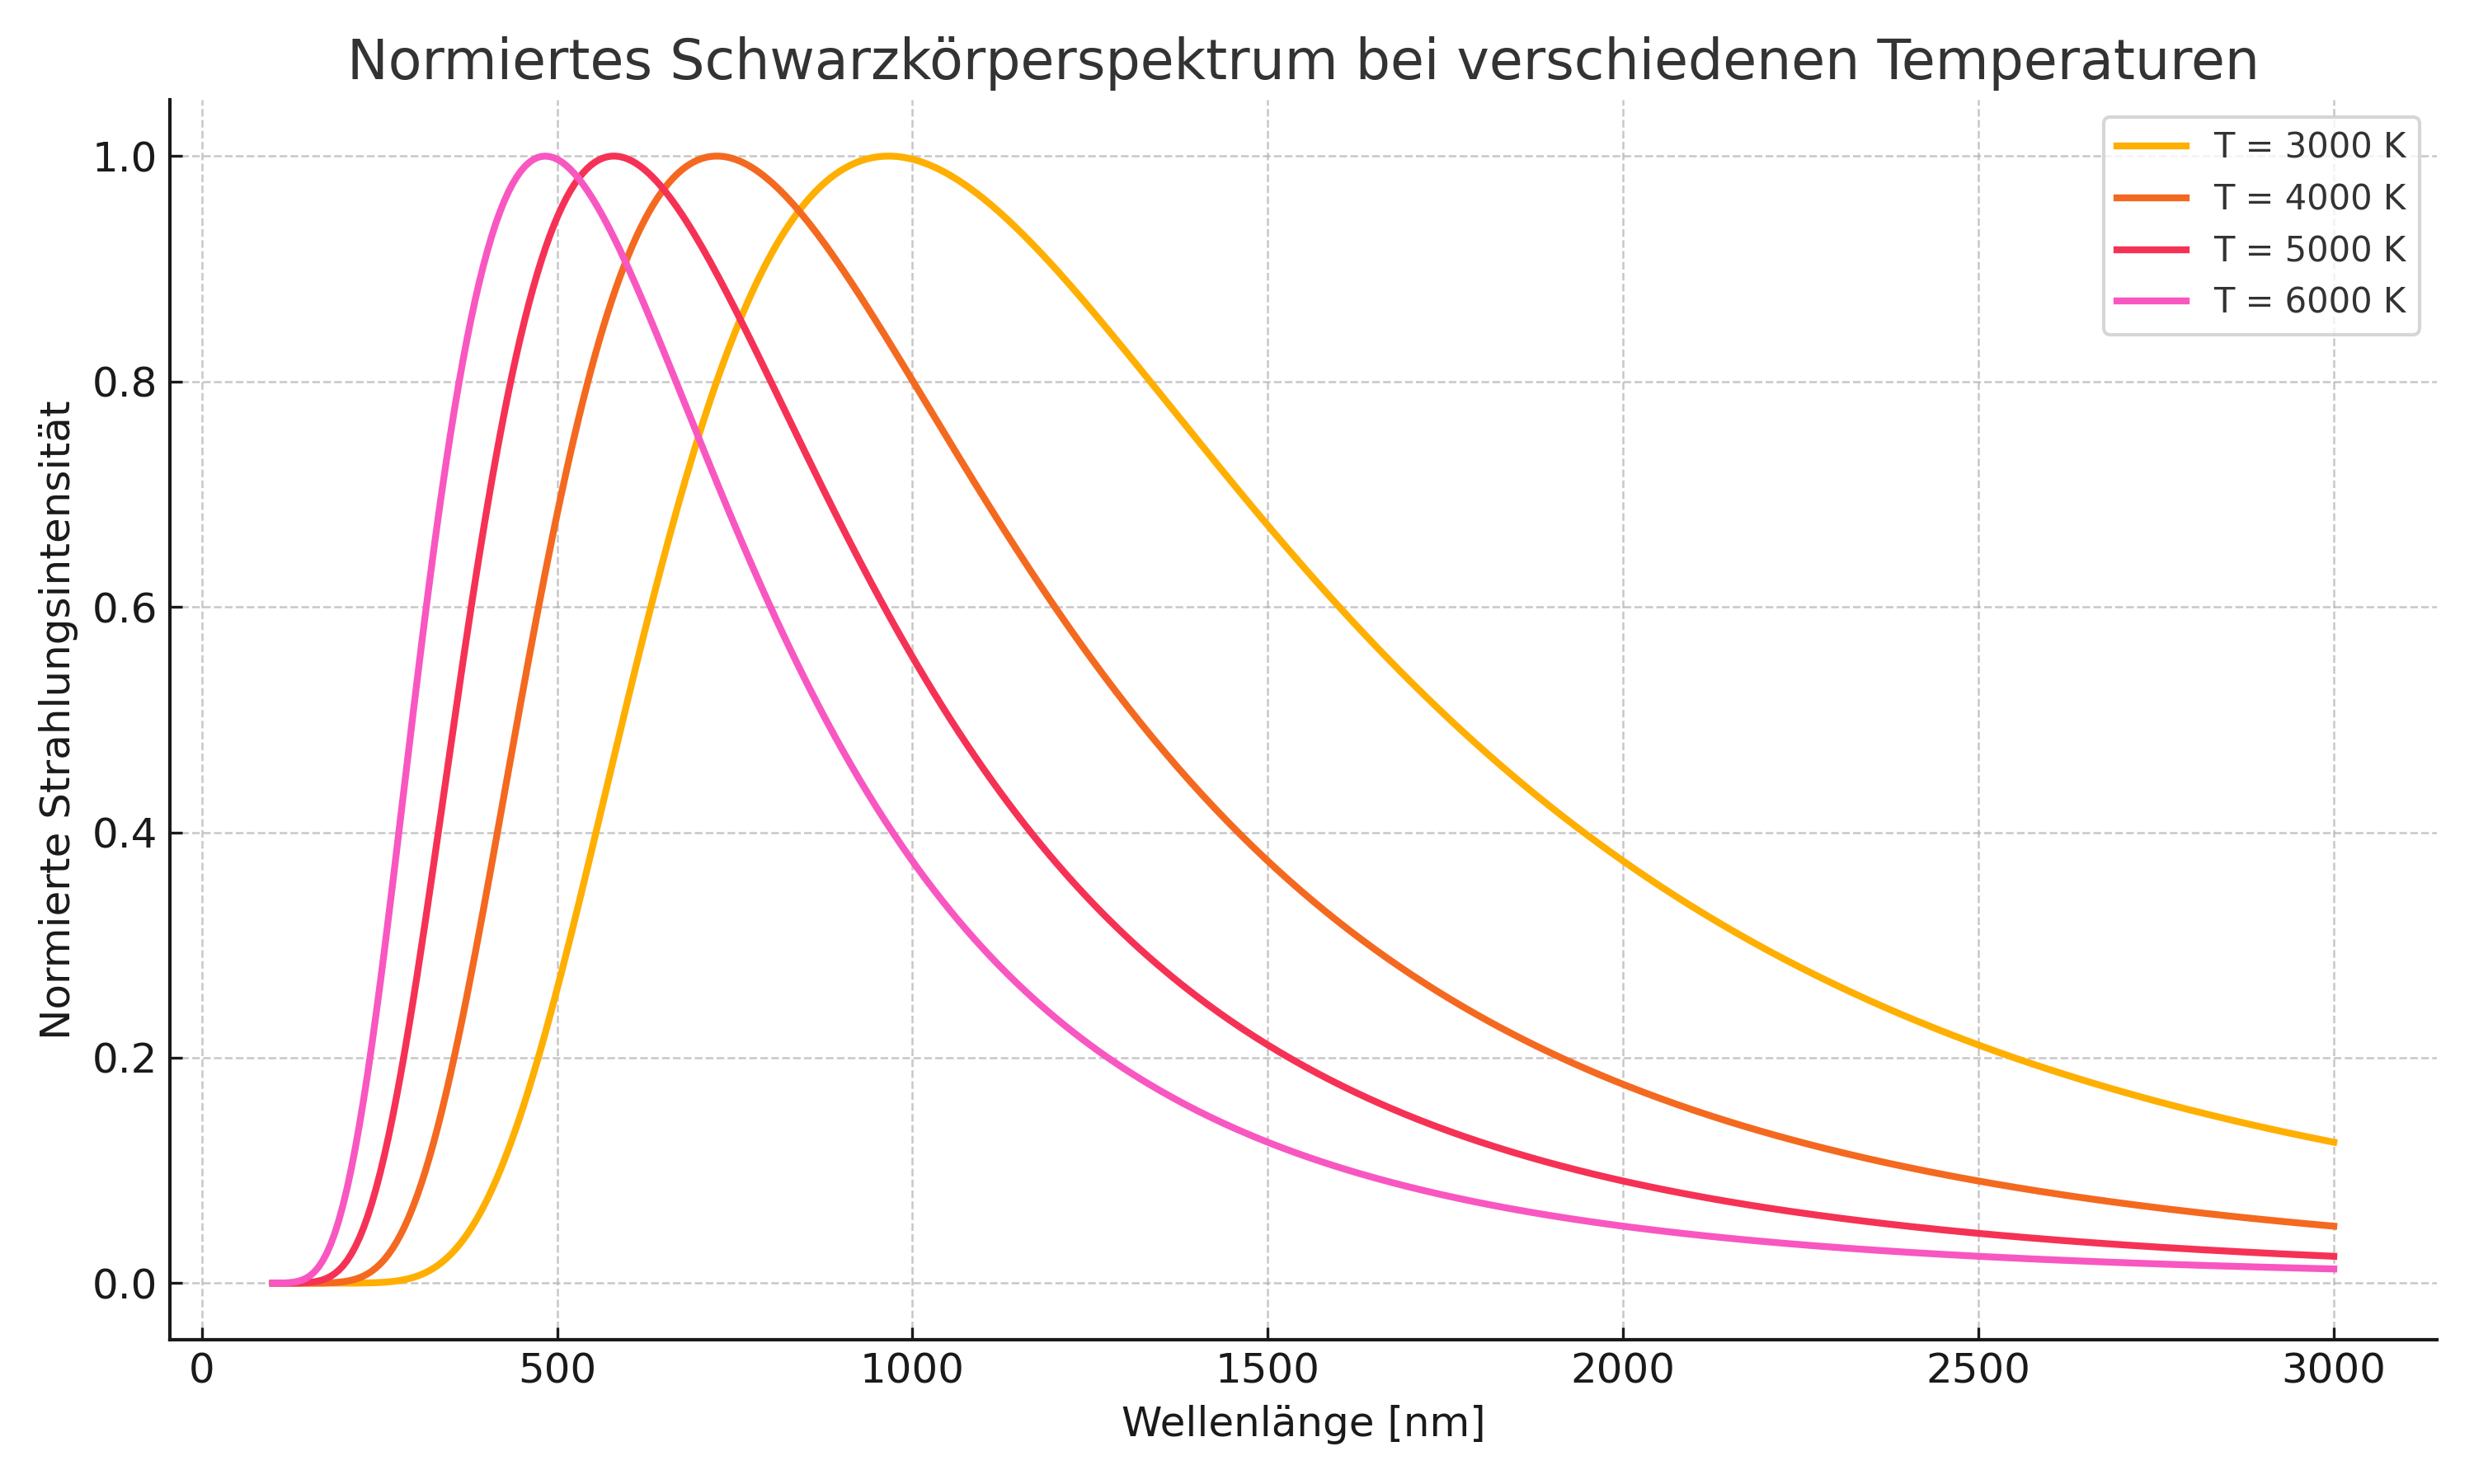
\includegraphics[width=0.85\textwidth]{bilder/schwarzer_koerper_spektrum.png}
	\caption{Normalized blackbody spectrum for different temperatures. The maximum shifts to shorter wavelengths as the temperature increases (Wien’s displacement law).}
	\label{fig:schwarzerkoerper}
\end{figure}
\subsubsection{Procedure of the Cavity Experiment}

To experimentally investigate thermal radiation, so-called \emph{cavity radiators}\index{Cavity Radiator} are used. They serve as nearly ideal realizations of a blackbody. The typical setup consists of a solid metal block with an inner cavity and a small opening to the outside world.

Radiation entering through this opening is reflected many times at the walls and is almost completely absorbed. Conversely, a tiny portion of the internal equilibrium radiation exits through the opening – this corresponds almost exactly to the theoretical blackbody radiation at the block’s temperature \( T \).  

The radiation emerging from the opening is studied with a spectrometer.\index{Spectrometer} The resulting spectrum shows the typical blackbody curve: an intensity profile with a maximum that shifts with temperature (Wien’s displacement law), and a characteristic drop in the ultraviolet region. These results fundamentally contradicted classical physics and ultimately led to the development of quantum theory.

\begin{figure}[H]
	\centering
	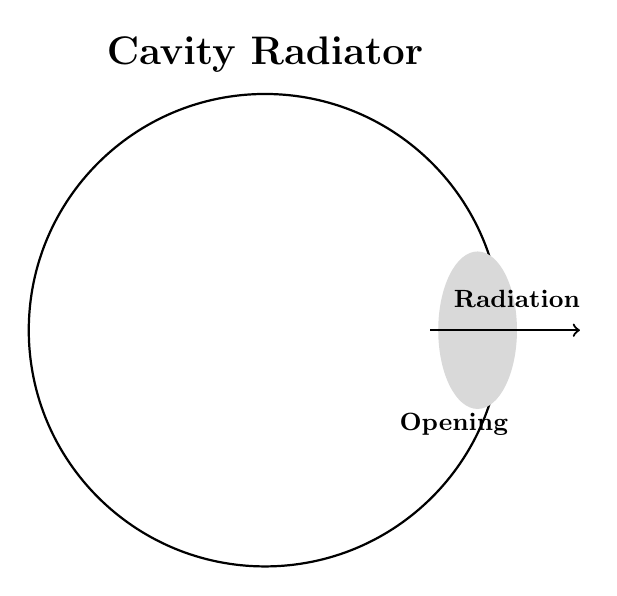
\begin{tikzpicture}
		% Cavity
		\draw[thick] (0,0) circle(3);
		% Opening (right side)
		\fill[gray!30] (2.7,0) ellipse (0.5 and 1.0);
		% Outgoing radiation
		\draw[->, thick] (2.1,0) -- (4,0);
		\node at (3.2,0.4) {\small \textbf{Radiation}};
		% Labels
		\node at (2.4,-1.2) {\small \textbf{Opening}};
		\node at (0,3.5) {\Large \textbf{Cavity Radiator}};
	\end{tikzpicture}
	\caption{Model of a cavity radiator producing nearly ideal blackbody radiation.}
\end{figure}
\subsection{Failure of the Classical Theory – \newline the Rayleigh–Jeans Law}\index{Rayleigh–Jeans Law}

In the 19th century, Lord Rayleigh and Sir James Jeans\index{Rayleigh, Lord}\index{Jeans, James} attempted to describe blackbody radiation using classical electrodynamics and statistical mechanics.\index{Statistical Mechanics} They treated standing electromagnetic waves in a cavity as harmonic oscillators and calculated the energy distribution by applying the equipartition principle of classical thermodynamics.\index{Equipartition Principle}
\newpage
\noindent
The result was the so-called \emph{Rayleigh–Jeans Law}, which gives the spectral energy density as a function of wavelength \( \lambda \) and temperature \( T \):

\[
u(\lambda, T) = \frac{8 \pi k T}{\lambda^4}
\]

Here:
\begin{itemize}
	\item \( u(\lambda, T) \): radiation energy per wavelength interval and volume,
	\item \( k \): Boltzmann constant,\index{Boltzmann Constant}
	\item \( T \): absolute temperature.
\end{itemize}

For long wavelengths the formula yields reasonable results and agrees well with experimental data. But at short wavelengths the expression diverges to infinity – leading to an unphysical, infinite energy density:

\[
\lim_{\lambda \to 0} u(\lambda, T) \to \infty
\]

This problem became known as the \emph{ultraviolet catastrophe}.\index{Ultraviolet Catastrophe} It stood in fundamental contradiction to experimental observations (see Fig.~\ref{fig:schwarzerkoerper}), where radiation in the UV region does not increase but instead falls off sharply.

This catastrophe revealed the limitations of classical physics. A new idea was required to explain the observations – and it came from Max Planck.  
(The derivation via mode counting in a cavity and the classical equipartition principle is presented in Appendix~A, Section~\ref{anhangA:rayleigh}.)
\subsection{Failure of the Classical Theory – \newline Wien’s Radiation Law}\index{Wien’s Radiation Law}

Even before Planck, Wilhelm Wien\index{Wien, Wilhelm} in 1896 provided an approximation for the radiation spectrum of blackbodies in the short-wavelength range. He derived the so-called \emph{Wien’s Radiation Law} from thermodynamic arguments and dimensional analysis – but without the quantum concept we know today.
\newpage
\noindent
The spectral energy density in wavelength form is given by:

\[
u(\lambda, T) = \frac{c_1}{\lambda^5} \exp\left(-\frac{c_2}{\lambda T}\right)
\]

with:
\begin{itemize}
	\item \( u(\lambda, T) \): energy per wavelength interval and volume,
	\item \( \lambda \): wavelength,\index{Wavelength}
	\item \( T \): absolute temperature,
	\item \( c_1 = 2\pi h c^2 \), \( c_2 = \tfrac{hc}{k} \): constants from Planck units (fully understood only later).\index{Planck Units}
\end{itemize}

Wien’s law describes the radiation distribution in the high-frequency range (\( \lambda \to 0 \)) very well and predicts an exponential decrease in intensity. In the long-wavelength range (\( \lambda \gg 1\ \mu\mathrm{m} \)), however, it deviates significantly from the measurements.

Wilhelm Wien received the Nobel Prize in 1911 for his contributions to radiation theory. His law was an important step toward Planck’s complete theory.  
(The mathematical derivation of Wien’s radiation law is given in Appendix~A; see Section~\ref{anhangA:wien}.)

\vspace{1em}
\begin{tcolorbox}[didaktikbox, title=Why Does the Classical Theory Fail?]
	\label{box:klassik-versagt}
	The Rayleigh–Jeans law correctly describes thermal radiation at low frequencies – but at high frequencies it gives absurd results:
	
	\begin{itemize}
		\item Intensity rises without bound – the higher the frequency, the greater the radiation.
		\item This “ultraviolet catastrophe” contradicts all observations.
		\item The cause: classical physics assumes that every mode in the cavity can absorb unlimited energy.
	\end{itemize}
	
	This assumption fails in reality. Only the quantization of energy – as introduced by Planck – explains why high frequencies are suppressed.
\end{tcolorbox}
\subsection{Emergence of Planck’s Radiation Law}\index{Planck’s Radiation Law}

At the end of the 19th century, describing the radiation of a blackbody posed a fundamental problem for theoretical physics. Empirically, the spectral energy density \( I(\lambda, T) \) was well known, but no theory could correctly explain the entire spectrum.

\subsubsection{The Crisis of Classical Physics}

Classical physics could only explain limiting cases:

\begin{itemize}
	\item For large wavelengths (\(\lambda \to \infty\)), the \textbf{Rayleigh–Jeans law}\index{Rayleigh–Jeans Law} was valid:
	\[
	I(\lambda, T) = \frac{8\pi c}{\lambda^4} \cdot kT
	\]
	This law, however, led to an unphysical divergence at short wavelengths – the so-called \textbf{ultraviolet catastrophe}.\index{Ultraviolet Catastrophe}
	
	\item For short wavelengths (\(\lambda \to 0\)), the \textbf{Wien’s law}\index{Wien’s Radiation Law} was known:
	\[
	I(\lambda, T) = c_1 \lambda^{-5} \cdot e^{-c_2/(\lambda T)}
	\]
	Yet it failed in the long-wavelength region.
\end{itemize}

\subsubsection{Planck’s Interpolation Approach}

Max Planck\index{Planck, Max} was familiar with both limiting laws and searched for a mathematical function that could interpolate across the entire observed curve. In October 1900, this led him to his famous formula:
\begin{align}
	I(\lambda, T) = \frac{2hc^2}{\lambda^5} \cdot \frac{1}{e^{hc/(\lambda kT)} - 1}
\end{align}

with:
\begin{itemize}
	\item \( h \): Planck’s constant\index{Planck’s Constant}
	\item \( c \): speed of light\index{Speed of Light}
	\item \( k \): Boltzmann constant\index{Boltzmann Constant}
	\item \( T \): absolute temperature
\end{itemize}

(The detailed derivation of Planck’s radiation law using energy quantization is presented in Appendix~A, Section~\ref{anhangA:planck}.)

\subsubsection{Remark on the Meaning of \( h \)}

Planck initially regarded his formula as a \textbf{mathematical interpolation}, not as the expression of a fundamental natural constant. He introduced \( h \) to fit the curve – without realizing the revolutionary consequences. Only Albert Einstein\index{Einstein, Albert} recognized its deeper meaning in 1905 within the framework of his light quantum hypothesis.

\vspace{-0.3em}
\begin{tcolorbox}[physikbox,title={Max Planck – Scientific Autobiography \cite{planck1948}}]
	\label{box:planck-zitat}
	“I had the feeling that I had introduced something monstrous against my will.”
\end{tcolorbox}

\vspace{1em}
\begin{tcolorbox}[mathebox, title={Planck’s Radiation Law: A Mathematical Interpolation \cite{Hoffmann2008}}]
	\label{box:planck-interpolation}
	At the end of 1900, Max Planck was searching for a function to correctly describe the observed blackbody radiation curves. He combined known limiting laws (Wien for high, Rayleigh for low frequencies) and developed an interpolation formula that later became known as Planck’s radiation law:
	
	\begin{align}
		I(\nu, T) = \frac{8\pi \nu^2}{c^3} \cdot \frac{h\nu}{e^{h\nu/kT} - 1}
	\end{align}
	
	At the time, he himself was unaware of the deeper meaning of the constant \( h \) – for him it was a mathematical tool. Only later did Einstein, with his light quantum hypothesis of 1905, interpret this formula as evidence of a fundamental quantization of nature.
\end{tcolorbox}
\newpage
\noindent
\subsubsection{Important Historical Insight}
\vspace{1em}
\begin{tcolorbox}[didaktikbox,title=Important Historical Insight {\cite{Hoffmann2008}}]
	\label{box:geschichte-planck}
	On December 14, 1900, Max Planck presented his famous radiation formula to the Physical Society. Today this day is regarded as the \textit{“birthday of quantum physics”}. Yet neither Planck nor his audience recognized the significance of the discovery at the time.
	
	\medskip
	\textbf{Quote:} 
	\begin{quote}
		“Although none of the scientists present – including Planck himself – were aware of the meaning and scope of the formula or the constant. Planck’s result was initially seen merely as a formula that correctly represented the radiation data.”
	\end{quote}
	
	As Hoffmann points out, the revolution only became clear through Einstein’s light quantum hypothesis (1905) and the critical analysis of Planck’s law by Einstein and Ehrenfest. Planck himself spoke of a fundamental upheaval only years later.
\end{tcolorbox}
\index{Quantum Physics}
\newpage
\noindent
\subsubsection{Graphical Comparison of the Three Radiation Laws}

The following figure shows the spectral energy density of blackbodies as a function of wavelength. It compares the classical Rayleigh–Jeans law, Wien’s radiation law, and the full Planck law. The diagram clearly illustrates:

\begin{itemize}
	\item The Rayleigh–Jeans law diverges in the UV region.
	\item Wien’s law is valid only in the short-wavelength region.
	\item Only Planck’s law correctly describes the entire spectrum.
\end{itemize}

\begin{figure}[H]
	\centering
	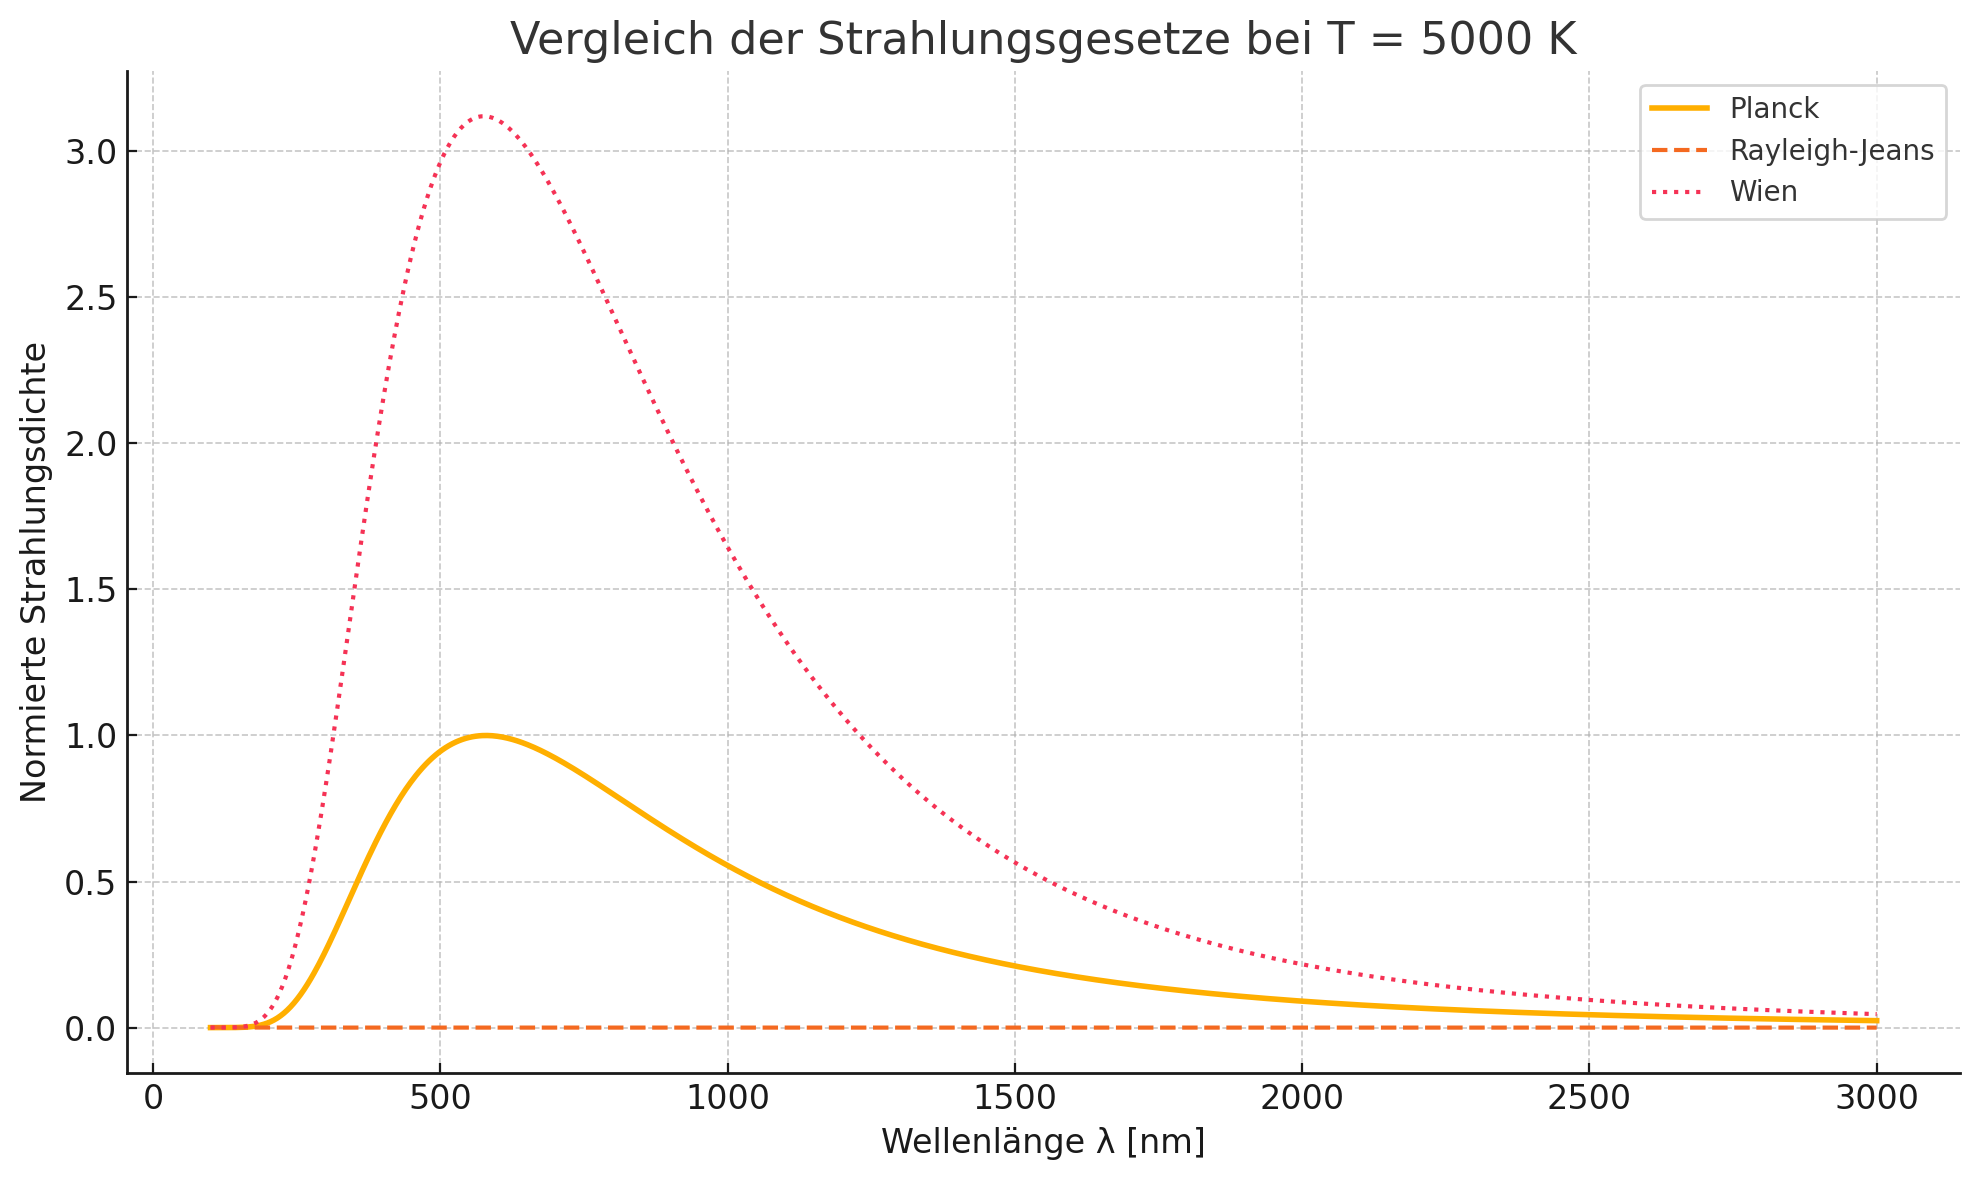
\includegraphics[width=0.85\textwidth]{bilder/strahlungsgesetze.png}
	\caption{Comparison of the three radiation laws. Only Planck’s law agrees with experimental data across the entire spectrum.}
	\label{fig:strahlungsgesetze}
\end{figure}

\subsubsection{Conclusion}

\begin{itemize}
	\item The error of the classical theory is not only large but catastrophic.
	\item The deviation at short wavelengths amounts to several orders of magnitude.
	\item Only Planck’s law explains the entire spectrum correctly – by quantizing energy.
\end{itemize}
\subsection{The Photoelectric Effect and Einstein’s Light Quantum}\index{Photoelectric Effect}

In 1905, Einstein went a step further: not only the emission of energy, but light itself was quantized. He postulated that a light quantum (photon) carries the energy \( E = h\nu \).\index{Einstein, Albert} Only if this energy exceeds the work function \( A \) can an electron be emitted:  
\[
E_{\text{kin}} = h\nu - A
\]
This explained experimental observations that were incompatible with the wave theory – in particular the frequency dependence of the electron energies.\index{Work Function}

\begin{tcolorbox}[physikbox, title={Einstein (1905)\cite{einstein_lichtquanten}}]
	\label{box:einstein-lichtquant}
	“The generation of light does not occur everywhere along the wavefront uniformly, but only at certain places, at individual points.”
	
	\textbf{Comment:} Here Einstein already describes the quantization of light – the starting point of photon theory.
\end{tcolorbox}
\vspace{1em}
\index{Light Quantum Hypothesis}

(A detailed derivation of the photoelectric equation can be found in Appendix~A, Section~\ref{anhangA:photoeffekt}.)
\subsection{First Reactions and Significance}

The idea that light possesses not only wave properties but also particle properties was difficult for many physicists at the beginning of the 20th century to accept. The wave theory of light had seemed fully confirmed by interference and diffraction experiments as well as by Maxwell’s electrodynamics.\index{Wave Theory of Light} Albert Einstein’s light quantum theory of 1905 – the radical thesis that light consists of discrete energy packets (later called \emph{photons}) – contradicted this established view.

Einstein himself was aware of the explosive nature of his hypothesis and described it as a “heuristic point of view.” Yet the concept was more than a mere computational trick – it fully explained the photoelectric effect and led to precise, experimentally testable predictions.

A striking example of the initial skepticism was Robert A. Millikan.\index{Millikan, Robert A.} Although in 1916 he himself confirmed the energy formula \( E = h \nu \) with high precision in a series of experiments, he long remained critical of the light quantum concept:

Only decades later did the light quantum hypothesis become accepted as a fundamental part of quantum physics – especially after phenomena such as \emph{Compton scattering} (1923) confirmed the momentum nature of the photon.\index{Compton Scattering}


The introduction of the photon revolutionized not only optics but was also crucial for:
\begin{itemize}
	\item the development of \emph{quantum mechanics},\index{Quantum Mechanics}
	\item the understanding of \emph{atoms and molecules},\index{Atom}\index{Molecule}
	\item the theory of \emph{quantum electrodynamics (QED)},\index{Quantum Electrodynamics (QED)}
	\item as well as numerous \emph{technological applications} (lasers, photodetectors, solar cells, quantum computers).\index{Laser}\index{Photodetector}\index{Solar Cell}\index{Quantum Computer}
\end{itemize}

Today the photon is not merely a theoretical construct, but a real object, demonstrated in countless experiments and used in technology – a \emph{quantum of the electromagnetic interaction}.\index{Electromagnetic Interaction}

\vspace{1em}
\begin{tcolorbox}[physikbox, title=Robert A. Millikan on Einstein (1916) \cite{millikan_1916}]
	\label{box:millikan-einstein}
	\emph{“Einstein’s photoelectric equation … cannot in my judgment be looked upon at present as resting upon a satisfactory theoretical foundation.”}
	
	\vspace{6pt}
	\textbf{Comment:} Despite his experimental confirmation of Einstein’s formula, Millikan initially rejected the light quantum concept – a striking example of how deeply rooted theoretical convictions cannot be immediately overturned, even by clear experimental evidence.
\end{tcolorbox}
\subsection{Conclusion}
\vspace{1em}
\begin{tcolorbox}[hypobox, title={What If There Were No Quantization?}]
	\label{box:hypo-keine-quanten}
	Without the assumption that energy can only be absorbed or emitted in discrete portions ($E = nhf$):\index{Quantization}
	\begin{itemize}
		\item Fundamental experiments such as blackbody radiation and the photoelectric effect would have remained unexplained.
		\item Classical physics would have collapsed under the contradictions with reality.
		\item No modern understanding of the interaction between light and matter would have developed.
	\end{itemize}
	Quantization was the first step toward a new physical worldview. It is not optional – it is essential for understanding the photon.
\end{tcolorbox}

